
\begin{frame}{von Neumann Architecture}
  \begin{columns}
    \begin{column}{0.5\textwidth}
      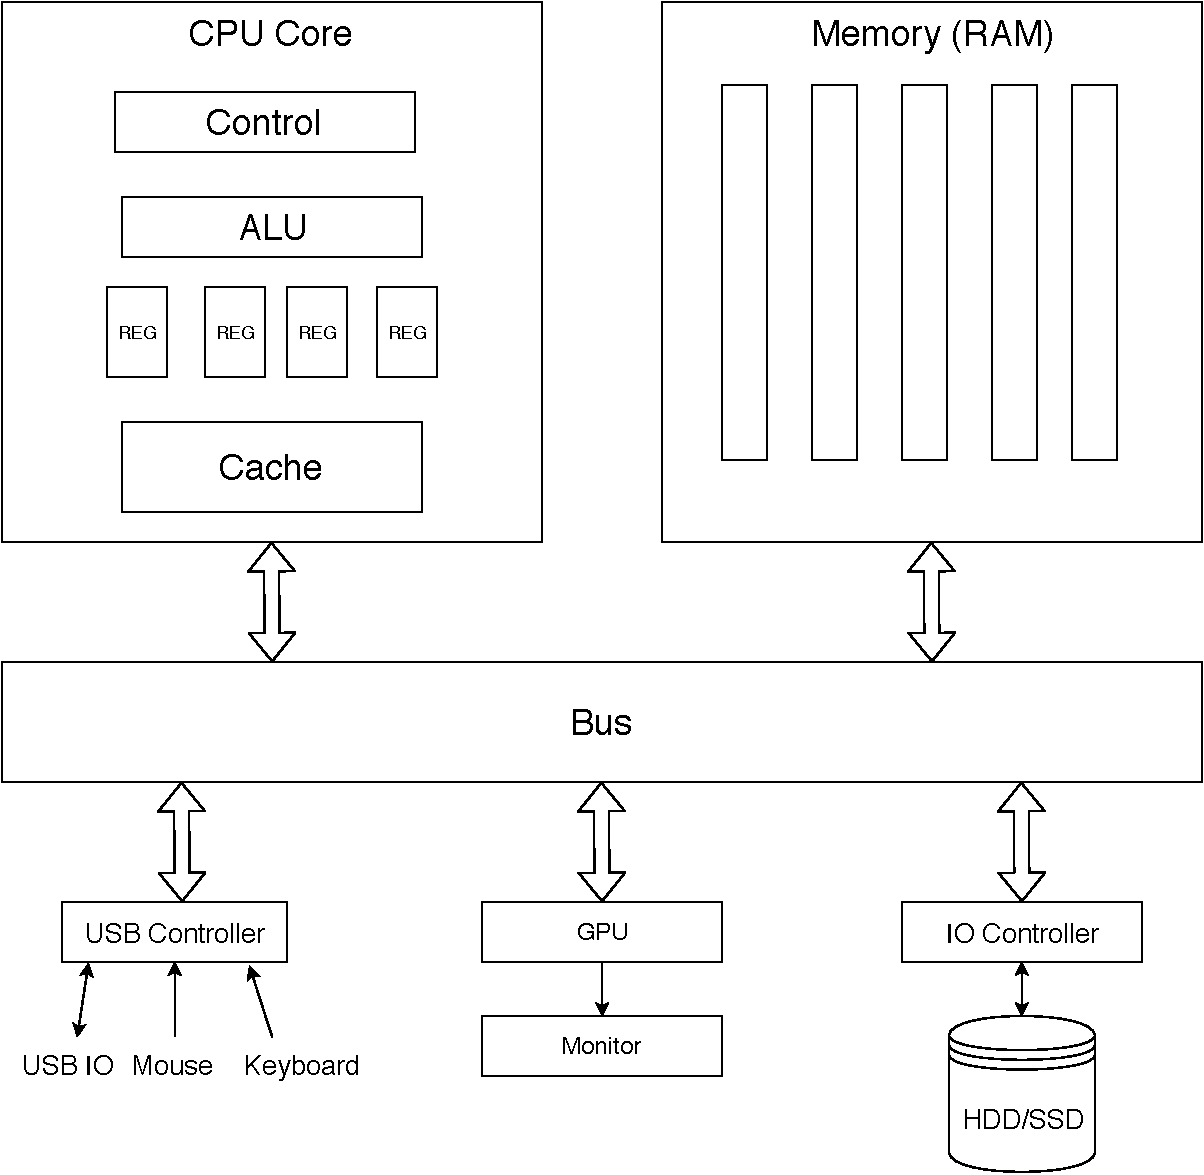
\includegraphics[width=\textwidth]{pic/VNeumann}
    \end{column}
    \begin{column}{0.5\textwidth}
  \begin{itemize}
  \item Data and code stored in the same memory $\Rightarrow$ encoded in the same way, stored as binary numbers
  \item Instruction cycle:
    \begin{itemize}
    \item
      Instruction decode: determine operation and operands
    \item
      Get operands from memory
    \item
      Perform operation
    \item
      Write results back
    \item
      Continue with next instruction
    \end{itemize}
  \end{itemize}

      
    \end{column}
  \end{columns}
  \begin{center}
  \end{center}

\end{frame}

\begin{frame}{Contemporary CPU Architecture}

  \begin{itemize}
    \tightlist
  \item
    Operations can be performed speculatively
  \item
    On-Core parallelism: multiple operations simultaneously 
  \item 
    Multicore  parallelism
  \item
    Operands can be in memory, cache, register
  \item
    Results may need to be coordinated with other processing elements
  \end{itemize}

  \begin{center}
    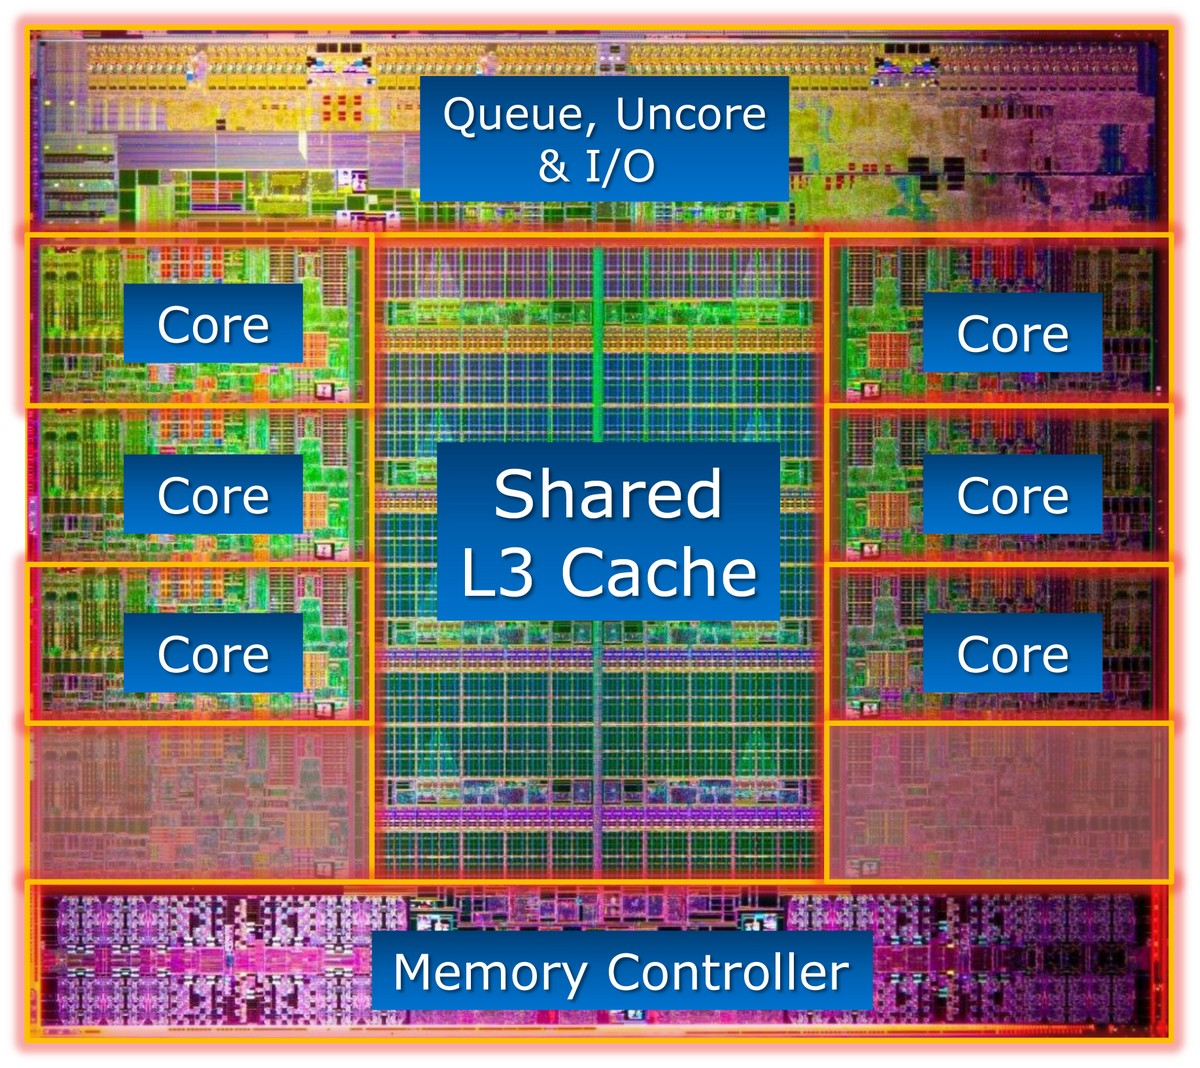
\includegraphics[width=0.6\textwidth]{pic/die}

    {\scriptsize Modern CPU. From: \url{https://www.hartware.de/review_1411_2.html}}
  \end{center}

\end{frame}

\begin{frame}{Modern CPU core functionality}

  \begin{itemize}
    \tightlist
  \item Clock: ``heartbeat'' of CPU
  \item
    Traditionally: one instruction per clock cycle
  \item
    Modern CPUs: Multiple floating point units,
    complex instructions, e.g.
    one multiplication + one addition as single instruction

    \begin{itemize}
      \tightlist
    \item
      Peak performance is several operations /clock cycle
    \item
      Only possible to obtain with highly optimized code
    \end{itemize}
  \item
    Pipelining

    \begin{itemize}
      \tightlist
    \item
      A single floating point instruction takes several clock cycles to
      complete:
    \item
      Subdivide an instruction:

      \begin{itemize}
        \tightlist
      \item
        Instruction decode
      \item
        Operand exponent align
      \item
        Actual operation
      \item
        Normalize
      \end{itemize}
    \item
      Pipeline: separate piece of hardware for each subdivision
    \item
      Like assembly line
    \end{itemize}
  \end{itemize}

\end{frame}



\begin{frame}[fragile]{Memory Hierachy}
  \begin{itemize}
  \item
    Main memory access is slow compared to the processor
    
    \begin{itemize}
      \tightlist
    \item
      100--1000 cycles latency before data arrive
    \item
      Data stream maybe 1/4 floating point number/cycle;
    \item
      processor wants 2 or 3
    \end{itemize}
  \item
    Faster memory is expensive
  \item
    \emph{Cache} is a small piece of fast memory for intermediate storage
    of data
  \item
    Operands are moved to CPU \emph{registers} immediately before
    operation
  \item Memory hierarchy:
    \begin{center}
      Registers in different cores\\
      Fast on-CPU cache memory (L1, L2, L3)\\
      Main memory
    \end{center}
    
  \item
      Registers are filled with data from main memory via cache:
  \begin{itemize}
    \tightlist
  \item
    L1 Cache: Data cache closest to registers
  \item
    L2 Cache: Secondary data cache, stores both data and instructions
  \item
    Data from L2 has to go through L1 to registers
  \item
    L2 is 10 to 100 times larger than L1
  \item
    Some systems have an L3 cache, $\approx$10x larger than L2
  \end{itemize}

  \end{itemize}  
\end{frame}




\begin{frame}{Cache line}

  \begin{itemize}
  \item
    The smallest unit of data transferred between main memory and the
    caches (or between levels of cache)
  \item
    N sequentially-stored, multi-byte words (usually N=8 or 16).
  \item
    If you request one word on a cache line, you get the whole line

    \begin{itemize}
      \tightlist
    \item
      make sure to use the other items, you've paid for them in bandwidth
    \item
      Sequential access good, ``strided'' access ok, random access bad
    \end{itemize}
  \item
    Cache hit: location referenced is found in the cache
  \item
    Cache miss: location referenced is not found in cache

    \begin{itemize}
      \tightlist
    \item
      triggers access to the next higher cache or memory
    \end{itemize}
  \item
    Cache thrashing

    \begin{itemize}
      \tightlist
    \item
      Two data elements can be mapped to the same cache line: loading the
      second ``evicts'' the first
    \item
      Now what if this code is in a loop? ``thrashing'': really bad for
      performance
    \end{itemize}
  \item
    Performance is limited by data transfer rate

    \begin{itemize}
      \tightlist
    \item
      High performance if data items are used multiple times
    \end{itemize}
  \end{itemize}

\end{frame}

%%% Local Variables:
%%% mode: latex
%%% TeX-master: "l01-intro"
%%% End:
